\documentclass{article}

\usepackage[final, nonatbib]{neurips_2024}

\usepackage{float}

\usepackage[utf8]{inputenc} % UTF-8 giriş desteği
\usepackage[T1]{fontenc}    % T1 font kullanımı
\usepackage{booktabs}       % Profesyonel tablo kalitesi
\usepackage{amsfonts}       % Matematik sembolleri
\usepackage{nicefrac}       % Kompakt semboller (1/2, vb.)
\usepackage{microtype}      % Mikro-tipografi
\usepackage{xcolor}         % Renk desteği
\usepackage{graphicx}       % Grafik ekleme
\usepackage{amsmath}        % Gelişmiş matematiksel ifadeler
\usepackage{threeparttable} % Üç parçalı tablolar
\usepackage[normalem]{ulem} % Altı çizili metin
\useunder{\uline}{\ul}{}    % Altı çizili metin için özel stil

\title{Tokenizasyonun Yeniden Ele Alınması: Çok Dilli NLP'de Verimlilik ve Dilbilimsel Bütünlüğün Dengesi}

\author{
M. Ali Bayram$^1$, Ali Arda Fincan$^2$, Ahmet Semih Gümüş$^2$, Sercan Karakaş$^3$, Banu Diri$^1$\\
$^1$Yıldız Teknik Üniversitesi, $^2$Yeditepe Üniversitesi, $^3$OpenAI \\
\texttt{malibayram20@gmail.com}
}

\begin{document}

\maketitle

\begin{abstract}
  Tokenization is a critical preprocessing step in natural language processing (NLP), shaping how effectively large language models (LLMs) capture linguistic and semantic nuance. This paper presents a comprehensive framework for tokenization standards that prioritize morphological and semantic integrity, especially for morphologically complex and low-resource languages. Using Turkish as a case study, we evaluate eight LLM-derived tokenizers on a subset of the Massive Multitask Language Understanding (MMLU) benchmark. Our analysis goes beyond conventional efficiency metrics—such as vocabulary size, token count, and processing speed—by incorporating linguistic token percentages and semantic purity to assess how faithfully tokenizers preserve linguistic structure. The results highlight that language-specific tokenization strategies substantially improve downstream performance, even when training data is limited, and show that larger model parameters do not inherently yield better tokenization or enhanced results. These findings underscore the need to balance computational efficiency with linguistic alignment, tailoring tokenization methods to the morphological properties of each language. The proposed framework is adaptable to various linguistic contexts, guiding the development of tokenizers that improve model accuracy, robustness, and versatility. Future work will explore advanced morphological analysis, domain-specific customization, and cross-linguistic comparisons to further refine tokenization practices and advance the state of multilingual NLP.
  
  \textbf{Keywords:} Tokenization Standards, Morphological Integrity, Semantic Fidelity, Low-Resource Languages, Multilingual NLP, Morphologically Complex Languages
  \end{abstract}

\newenvironment{ozet}{
\begin{center}
\begin{minipage}{0.85\textwidth} % Sayfanın %85 genişliği kadar
\section*{Özet}
}{
\end{minipage}
\end{center}
}

\begin{ozet}
  Tokenizasyon, doğal dil işleme (NLP) alanında, büyük dil modellerinin (LLM'ler) dilbilimsel ve anlamsal detayları yakalama başarısını doğrudan şekillendiren kritik bir ön işleme adımıdır. Bu çalışma, özellikle morfolojik olarak zengin ve düşük kaynaklı dillerde, morfolojik ve anlamsal bütünlüğü önceliklendiren tokenizasyon standartları için kapsamlı bir çerçeve sunmaktadır. Örnek çalışma olarak Türkçeyi ele alarak, Massive Multitask Language Understanding (MMLU) benchmark'ının bir alt kümesinde sekiz farklı LLM tabanlı tokenizasyon yöntemi değerlendirilmiştir. Analizimiz, geleneksel verimlilik metriklerinin ötesine geçerek (örn. sözlük boyutu, token sayısı, işleme süresi), dilbilimsel token yüzdesi ve anlamsal saflık gibi metrikler üzerinden, tokenizasyonun dil yapısını ne derece doğru temsil ettiğini incelemiştir. Sonuçlar, dil spesifik tokenizasyon stratejilerinin, sınırlı eğitim verisi olduğunda dahi aşağı akış performansını önemli ölçüde iyileştirdiğini ve daha büyük model parametrelerinin her zaman daha iyi tokenizasyon veya sonuçlar sağlamadığını göstermektedir. Bu bulgular, hesaplama verimliliği ile dilbilimsel uyumu dengeleyerek tokenizasyon yöntemlerinin her dilin morfolojik özelliklerine göre uyarlanması gerektiğini vurgulamaktadır. Önerilen çerçeve, farklı dil bağlamlarına uyarlanabilir olup, model doğruluğunu, dayanıklılığını ve çok yönlülüğünü artıran tokenizasyon geliştirmeleri için bir rehber niteliğindedir.
  
  \textbf{Anahtar Kelimeler:} Tokenizasyon Standartları, Morfolojik Bütünlük, Anlamsal Saflık, Düşük Kaynaklı Diller, Çok Dilli NLP, Morfolojik Olarak Zengin Diller
\end{ozet}

\section{Giriş}

Tokenizasyon, doğal dil işleme (NLP) alanında, dil modellerinin etkili ve verimli çalışmasını doğrudan etkileyen kritik bir ön işleme adımıdır. Bu süreç, metni kelime, alt kelime veya karakter gibi daha küçük birimlere ayırmayı içerir ve bu birimler modeller için temel giriş verilerini oluşturur. Tokenizasyon, tüm dillerde evrensel bir gereklilik olmasına rağmen, morfolojik olarak zengin ve eklemeli dillerde, örneğin Türkçede, bu süreç daha karmaşık hale gelir. Türkçe gibi dillerde, tek bir kelime genellikle bir kök ve birden fazla ek içerir; her biri ayrı bir dilbilgisel veya anlamsal anlam taşır. Bu gibi durumlarda, standart tokenizasyon yöntemleri ince dilbilimsel özellikleri yakalamakta başarısız olabilir ve aşağı akış görevlerindeki performansı düşürebilir.

Son yıllarda, Byte Pair Encoding (BPE) ve SentencePiece gibi alt kelime tokenizasyon tekniklerindeki gelişmeler, dillerin karmaşık yapılarının daha iyi temsil edilmesinde önemli iyileştirmeler sağlamıştır. Bu yöntemler, kelimeleri daha küçük alt kelime birimlerine bölerek, modellerin nadir ve görülmemiş kelimelerle daha etkili bir şekilde başa çıkmasına olanak tanır. Örneğin, Arapça için geliştirilen \texttt{Aranizer-PBE-86k} tokenizatörü, dilin morfolojik inceliklerini etkili bir şekilde yakalayarak Türkçe gibi diğer dillerdeki benzer zorlukların üstesinden gelme konusunda önemli ipuçları sunmaktadır \cite{koubaa_githubcomriotu-labaranizer_2024}. Bu yöntemler, İngilizce gibi daha basit morfolojilere sahip dillerde dahi, özellikle veri kıtlığının olduğu senaryolarda, desen tanıma ve temsil verimliliğini artırmaktadır.

Tokenizasyon kalitesini değerlendirmek için iki kritik metrik vardır: \textit{token saflığı} ve bir dil için \textit{token yüzdesi}. Token saflığı, üretilen tokenların anlamlı dilbilimsel birimlere (ör. kökler, geçerli ekler veya anlamsal olarak tutarlı segmentler) ne derece uyduğunu ölçer. Yüksek bir token saflığı, kelimelerin anlamlı parçalarının tokenizasyon sırasında korunmasını sağlar, parçalanmayı en aza indirir ve modellerin dil kalıplarını daha etkili bir şekilde öğrenmesine olanak tanır. Belirli bir dilin token yüzdesi, örneğin Türkçe token yüzdesi (\%TR), bir dilin yapısına uygun olarak geçerli kelimeler veya dilbilimsel birimler olan tokenların oranını belirtir. Bu metrik, tokenizasyonun hedef dilin yapısına uygunluğunu sağlar ve geçersiz veya dilbilimsel olmayan tokenlardan kaynaklanan gürültüyü azaltır.

Bu metrikler, yalnızca morfolojik olarak zengin diller için değil, aynı zamanda İngilizce gibi tüm diller için evrensel olarak önemlidir. Yüksek token saflığı ve dil spesifik token yüzdesi, dil modellerinin sınırlı eğitim verisiyle dahi anlamlı kalıpları daha etkili bir şekilde öğrenmesine olanak tanır. Dilbilimsel birimlerin anlamsal bütünlüğünün korunması, modellerin büyük ölçekli veri setlerine ihtiyaç duymadan genelleme yapmasına ve aşağı akış görevlerinde daha iyi performans göstermesine yardımcı olur. Bu durum, özellikle düşük kaynaklı diller veya eğitim verisinin kısıtlı olduğu uzmanlaşmış alanlar için büyük önem taşımaktadır.

Son yıllardaki gelişmelere rağmen, tokenizasyon hızını, sözlük boyutunu ve dilbilimsel bütünlüğü dengeleme konusu halen bir zorluktur. Aşırı parçalanma, anlamsal anlamı seyreltebilirken, aşırı kaba tokenizasyon kritik dilbilimsel detayları gözden kaçırabilir. Bu denge, yalnızca Türkçe gibi morfolojik olarak zengin diller için değil, aynı zamanda daha basit dillerdeki performans ve verimlilik için de hayati öneme sahiptir \cite{neubeck_so_2024}.

Bu makale, Türkçe için MMLU benchmark'ını kullanarak tokenizasyon yöntemlerini değerlendirmektedir. Token saflığı, token yüzdesi, sözlük boyutu ve işleme hızı gibi metriklere dayalı analiz yaparak, Türkçe NLP görevleri için en etkili yaklaşımları belirlemeyi hedeflemektedir. Bu çalışmadan elde edilen bulgular, tüm dillerde optimize edilmiş tokenizasyon stratejilerinin geliştirilmesine katkıda bulunmakta ve NLP modellerinin doğruluğunu ve verimliliğini artırmaktadır.

\section{İlgili Çalışmalar}

Tokenizasyon, doğal dil işleme (NLP) alanında dil modellerinin performansı, verimliliği ve doğruluğunu doğrudan etkileyen temel bir role sahiptir. Son çalışmalar, dilbilimsel bütünlüğü, hesaplama verimliliğini ve model ölçeklenebilirliğini dengelemek amacıyla çeşitli tokenizasyon stratejilerini ve bunların aşağı akış etkilerini araştırmıştır.

\textit{Arabic Tokenizers Leaderboard} \cite{rashad_arabic_nodate}, Arapça'nın çeşitli lehçeleri ve yazım karmaşıklığının neden olduğu zorlukları vurgulayarak \texttt{rasaif-translations} ve \texttt{Moroccan Arabic Wikipedia} gibi datasetler kullanarak Arapça tokenizatörlerini karşılaştırmaktadır. Bu çalışmada kullanılan araçlardan biri olan \textit{AraNizer} \cite{koubaa_githubcomriotu-labaranizer_2024}, Byte Pair Encoding (BPE) ve SentencePiece gibi alt kelime tabanlı tekniklerden yararlanarak, Arapça’nın morfolojik inceliklerini daha iyi yakalamayı ve aşağı akış görevlerindeki performansı artırmayı amaçlamaktadır.

Benzer şekilde, \textit{NbAiLab Tokenizer Benchmark} \cite{rosa_nbailabtokenizer-benchmark_2024}, İskandinav dilleri için tokenizasyon stratejilerini değerlendirerek, çok dilli bağlamlarda dil spesifik adaptasyonların önemini vurgulamaktadır. Almanca için Diewald ve arkadaşları \cite{diewald_tokenizing_2022}, \texttt{KorAP-Tokenizer} ve \texttt{SoMaJo} gibi araçları değerlendirerek, büyük ölçekli metinler için yüksek doğruluk ve hesaplama verimliliği sağlamayı başarmıştır.

EuroLLM ekibi, çok dilli yapıların desteklenmesi için geniş sözlüklere sahip tokenizatörlerin tasarımının önemini vurgulayan önemli bir katkı sunmaktadır \cite{martins_eurollm_2024}. Byte Pair Encoding (BPE) ile birlikte byte fallback kullanan ve 128,000 parçalı bir sözlük içeren EuroLLM tokenizatörü, düşük "fertility" (kelime başına token sayısı) ile parametre verimliliği arasında bir denge sağlamaktadır. EuroLLM’nin, Mistral, LLaMA-3 ve Gemma tokenizatörleriyle yaptığı fertility karşılaştırmaları, geniş sözlüklerin hesaplama maliyetleri ile dil işleme yetenekleri arasındaki dengeyi anlamaya yönelik önemli bulgular sunmaktadır.

Verimlilik konusundaki ilerlemeler, GitHub’ın hızlı BPE uygulamasında da gözlemlenmiştir \cite{neubeck_so_2024}. Bu uygulama, milyarlarca token gerektiren görevlerde ölçeklenebilirliği artırarak, büyük ölçekli NLP görevleri için önemli bir performans artışı sağlamaktadır.

Rust ve arkadaşları \cite{rust_how_2021}, belirli dillere özel olarak uyarlanmış monolingual tokenizatörlerin, aşağı akış görev performansını önemli ölçüde artırdığını göstermektedir. Benzer şekilde, Lin ve arkadaşları \cite{lin_not_nodate}, tokenlara fayda puanı atayan ve yüksek faydalı tokenlar üzerinde seçici eğitim uygulayan Selective Language Modeling (SLM) yöntemini önermektedir. Bu yöntem, Türkçe gibi morfolojik olarak zengin dillerde anlamlı tokenların korunmasının kritik olduğu durumlarda özellikle yararlıdır.

Bu çalışmalar, dilbilimsel bütünlük, hesaplama verimliliği ve aşağı akış performansı arasında bir denge sağlayan tokenizasyon stratejilerinin gerekliliğini vurgulamaktadır. Bu çalışmada, Türkçe için tokenizatörler değerlendirilerek token saflığı, sözlük boyutu ve işleme hızı gibi metrikler kullanılmıştır. Çok dilli projelerden, özellikle EuroLLM'den elde edilen içgörüler entegre edilerek, morfolojik olarak zengin diller için tekniklerin optimize edilmesine katkıda bulunulmuştur.

\section{Yöntem}

Bu çalışma, morfolojik olarak zengin ve eklemeli dillere yönelik tokenizasyon stratejilerini değerlendirmeyi hedeflemekte olup, Türkçe bu bağlamda temsilci bir örnek olarak kullanılmaktadır. Ana odak Türkçe olsa da, yöntem diğer dillerdeki benzer tokenizasyon zorluklarına uyarlanabilir bir esneklikle tasarlanmıştır.

Bu değerlendirmeyi gerçekleştirmek için, çeşitli konuları kapsayan 6.200 çoktan seçmeli sorudan oluşan Türkçe MMLU veri seti kullanılmıştır \cite{bayram_turkish_nodate}. Bu veri seti, Hugging Face deposunda saklanan ön işlenmiş bir kaynaktan soruların ve cevapların çıkarılmasıyla hazırlanmıştır \cite{bayram_turkish_nodate}. Ortaya çıkan metin korpusu, Türkçe'de karşılaşılan çeşitli dilbilimsel yapıları geniş bir kapsama alanıyla içeren birleşik bir veri setine dönüştürülmüştür. Türkçe verileri kullanılarak geliştirilen bu çerçeve, benzer dil araçları ve kaynaklarının uygulanmasıyla diğer dillere de uyarlanabilir.

Bu çalışma kapsamında, tokenizasyonun hem hesaplama hem de dilbilimsel yönlerini değerlendirmek için çeşitli metrikler kullanılmıştır:

\textbf{Sözlük Boyutu:}  
Bir tokenizatörün üretebileceği benzersiz tokenların (ör. kelimeler, alt kelimeler, karakterler) toplam sayısını ifade eder. Örneğin, 50.000 sözlük boyutuna sahip bir tokenizatör \texttt{"cat"} veya \texttt{"run"} gibi tokenları, ayrıca \texttt{"run"} ve \texttt{"ning"} gibi alt kelime birimlerini içerebilir. Daha büyük sözlükler daha karmaşık dilbilimsel yapıları yakalayabilir, ancak aşırı büyük sözlükler karmaşıklığı ve bellek kullanımını artırabilirken, daha küçük sözlükler nadir kelimeleri yeterince temsil edemeyebilir.

\textbf{Toplam Token Sayısı:}  
Tokenizatör uygulandıktan sonra veri setinde üretilen toplam token sayısını ifade eder. Örneğin, \texttt{"I love programming languages"} cümlesi, boşluk tabanlı bir tokenizatörle [\texttt{"I"}, \texttt{"love"}, \texttt{"programming"}, \texttt{"languages"}] olarak ayrıştırıldığında dört token oluşur. Alt kelime tabanlı bir tokenizatör, [\texttt{"I"}, \texttt{"love"}, \texttt{"program"}, \texttt{"ming"}, \texttt{"languages"}] şeklinde beş token üretebilir. Daha düşük toplam token sayıları, daha kompakt temsiller anlamına gelebilir ve bu da verimliliği artırabilir.

\textbf{İşleme Süresi:}  
Veri setinin tamamını tokenize etmek için gereken süreyi (saniye cinsinden) ifade eder ve hesaplama verimliliğini yansıtır. Örneğin, bir milyon kelimelik bir korpus 3.2 saniyede işlenirse, işleme süresi 3.2 saniye olarak kaydedilir. Daha hızlı tokenizasyon, büyük ölçekli eğitimler ve gerçek zamanlı uygulamalar için avantajlıdır.

\textbf{Token Yüzdesi (\%TR):}  
Hedef dilde geçerli kelimelere veya morfemlere karşılık gelen tokenların oranını ölçen bir dilbilimsel metriktir. Örneğin, \texttt{"Cats are playing"} cümlesi [\texttt{"Ca"}, \texttt{"ts"}, \texttt{"are"}, \texttt{"play"}, \texttt{"ing"}] olarak tokenize edilirse, \texttt{"are"}, \texttt{"play"} ve \texttt{"ing"} geçerli dilbilimsel birimler olarak kabul edilir. Bu durumda:  
\[
\%TR = \frac{\text{Geçerli Tokenlar (3)}}{\text{Toplam Tokenlar (5)}} \times 100 = 60\%.
\]
Bu metrik, tokenizasyonun dilin morfolojisine uygunluğunu sağlar ve geçersiz segmentleri en aza indirir.

\textbf{Saf Token Yüzdesi (\%Pure):}  
Tokenların doğrudan anlamlı olup olmadığını ve daha küçük anlamlı parçalara ayrılıp ayrılamayacağını değerlendiren bir metriktir. Örneğin, \texttt{"The students are learning"} cümlesinde, \texttt{"The"} ve \texttt{"are"} saf tokenlardır, ancak \texttt{"students"} (\texttt{"student"} + \texttt{"s"}) ve \texttt{"learning"} (\texttt{"learn"} + \texttt{"ing"}) saf değildir, çünkü daha küçük birimlere ayrılabilirler. Eğer bir tokenizatör 100 benzersiz token üretmiş ve bunların 70’i saf token ise:  
\[
\%Pure = \frac{\text{Saf Tokenlar (70)}}{\text{Benzersiz Tokenlar (100)}} \times 100 = 70\%.
\]

Doğru morfolojik analiz ve token doğrulaması sağlamak için ITU Turkish NLP Web Service \cite{eryigit_itu_2014} ve Kalbur kütüphanesi \cite{aksoy_ahmetaxkalbur_2024} gibi dil araçlarından yararlanılmıştır. Diğer diller için benzer dil analiz araçları ve kurallara dayalı sistemler entegre edilebilir. İşleme süresi ve token sayıları gibi hesaplama metrikleri, Python betikleri ve Hugging Face Tokenizers kütüphanesi \cite{neubeck_so_2024} kullanılarak hesaplanmış ve bu, ölçeklenebilirliği ve uyarlanabilirliği sağlamıştır.

Tüm deneysel prosedürler, veri setleri ve yapılandırmalar çoğaltılabilirlik için belgelenmiştir. Bu çalışmada Türkçe birincil referans olarak kullanılmış olsa da, önerilen yöntem diğer dillere ve veri setlerine uygulanabilir bir yapı sunarak, farklı dilsel bağlamlarda tokenizasyon stratejilerini değerlendirmeye yönelik genel bir yaklaşım sunmaktadır.

\section{Sonuçlar ve Analiz}

Bu çalışmada, 1.605.376 karakter ve 198.193 kelimeden oluşan Türkçe MMLU veri seti üzerinde sekiz farklı tokenizatör değerlendirilmiştir \cite{bayram_turkish_nodate}. Hem dilbilimsel uyumu hem de hesaplama etkinliğini ölçmek amacıyla, Türkçe Token Yüzdesi (\%TR) ve Saf Token Yüzdesi (\%Pure) gibi dilbilimsel metrikler ile işleme süresi, model parametre boyutu ve MMLU skorları incelenmiştir. Analizlere model boyutunun dahil edilmesi, morfolojik olarak zengin diller için tokenizatör tasarımında yapılan ödünleşimleri daha ayrıntılı bir şekilde ortaya koymaktadır.

\begin{table}[H]
\centering
\caption{Tokenizatör Karşılaştırma Sonuçları}
\label{tab:tokenizer-benchmark}
\resizebox{\textwidth}{!}{
\begin{tabular}{|l|c|c|c|c|c|c|c|c|}
\hline
\textbf{Metrik} & \textbf{gemma-2} & \textbf{llama-3.1} & \textbf{EuroLLM} & \textbf{Qwen2.5} & \textbf{aya-exp} & \textbf{Mistral} & \textbf{Phi3.5} & \textbf{gpt4o} \\ \hline
Model Parametre (Milyar) & 27.2 & 70.6 & 9.2 & 7.6 & 32.3 & 12.2 & 3.8 & Bilinmiyor \\ \hline
MMLU Skoru (\%) & 72.10 & 70.42 & 51.29 & 61.68 & 70.66 & 46.89 & 29.37 & 84.84 \\ \hline
Sözlük Boyutu & 256,000 & 128,256 & 128,000 & 151,665 & 255,029 & 131,072 & 32,011 & 200,019 \\ \hline
Token Sayısı & 497,015 & 488,535 & 497,173 & 561,866 & 434,526 & 534,930 & 803,971 & 491,137 \\ \hline
İşleme Süresi (s) & 2.95 & 3.12 & 3.20 & 3.31 & 2.77 & 3.14 & 4.55 & 0.51 \\ \hline
Benzersiz Tokenlar & 6,383 & 6,823 & 5,226 & 5,752 & 8,562 & 4,354 & 3,640 & 7,615 \\ \hline
Türkçe Tokenlar & 3,104 & 3,125 & 2,457 & 2,320 & 4,338 & 1,971 & 1,599 & 3,209 \\ \hline
\%TR & 48.63 & 45.80 & 47.01 & 40.33 & 50.67 & 45.27 & 43.93 & 42.14 \\ \hline
Saf Tokenlar & 2,365 & 2,109 & 1,838 & 1,734 & 2,822 & 1,571 & 1,253 & 2,184 \\ \hline
\%Pure & 37.05 & 30.91 & 35.17 & 30.15 & 32.96 & 36.08 & 34.42 & 28.68 \\ \hline
\end{tabular}
}
\end{table}

Tablo~\ref{tab:tokenizer-benchmark}, sözlük boyutu, token sayıları, çalışma süresi ve dil spesifik uyum gibi metriklerin, modellerin performansıyla nasıl etkileşime girdiğini özetlemektedir. Özellikle, daha büyük parametre boyutlarının üstün sonuçlar garanti etmediği gözlemlenmiştir. Örneğin, \texttt{gemma-2} (27.2 milyar parametre), \texttt{llama-3.1} (70.6 milyar parametre) gibi oldukça büyük bir modelden daha yüksek Türkçe MMLU doğruluğu sağlamıştır. Bu durum, \texttt{gemma-2}’nin tokenizatörünün Türkçe morfolojisine daha iyi uyum sağladığını göstermektedir. Bunun aksine, İngilizce MMLU sıralamalarında \texttt{llama-3.1} üstün gelmektedir \cite{ai_llama_nodate}, bu da tokenizatör etkinliğinin dile bağımlılığını ortaya koymaktadır.

\texttt{gemma-2}, \%TR (48.63\%) ve \%Pure (37.05\%) açısından, \texttt{llama-3.1}’den (\%TR: 45.80\%, \%Pure: 30.91\%) daha yüksek değerler elde etmiştir. Bu durum, dil spesifik tokenizasyonun morfolojik yapıyı yakalamada ne kadar önemli olduğunu vurgulamaktadır. \texttt{aya-expanse} (32.3 milyar parametre) en yüksek \%TR (50.67\%) değerine ulaşsa da, MMLU skoru (70.66\%) dilsel uyumun hesaplama verimliliği ve görev optimizasyonu ile dengelenmesi gerektiğini göstermektedir.

Diğer yandan, \texttt{o200k-gpt40}, en yüksek MMLU skoruna (84.84\%) ve en hızlı işleme süresine (0.51s) sahip olmasına rağmen, göreceli olarak düşük bir \%TR (42.14\%) sergilemiştir. Bu durum, damıtma ve budama gibi optimizasyon tekniklerinin \cite{lacy_gpt-4o_2024,shakrapani_gpt_nodate}, dilsel bütünlük pahasına performans ve hızı artırabileceğini göstermektedir. Benzer şekilde, \texttt{Mistral} (12.2 milyar) ve \texttt{Phi3.5} (3.8 milyar) gibi daha küçük modeller, hem dilsel hem de hesaplama açısından düşük performans göstermiştir. Bu bulgular, sınırlı parametre boyutlarının, karmaşık morfolojileri etkili bir şekilde işlemek için daha gelişmiş tokenizasyon stratejilerine ihtiyaç duyduğunu göstermektedir.

Şekil~\ref{fig:model_comparison}, bu ödünleşimlerin çok boyutlu bir görselleştirmesini sunmaktadır. MMLU skorlarını \%TR'ye karşı çizerek, marker büyüklüğüyle parametre sayısını ve renk kodlamasıyla \%Pure'u temsil etmektedir. Bu görselleştirme, dilin morfolojik zenginliğini daha iyi yakalayan modeller ile daha büyük parametre sayısına veya belirli optimizasyonlara sahip modellerin genel performansta nasıl bir fark yarattığını holistik bir şekilde karşılaştırma olanağı sağlar.

\begin{figure}[H]
    \centering
    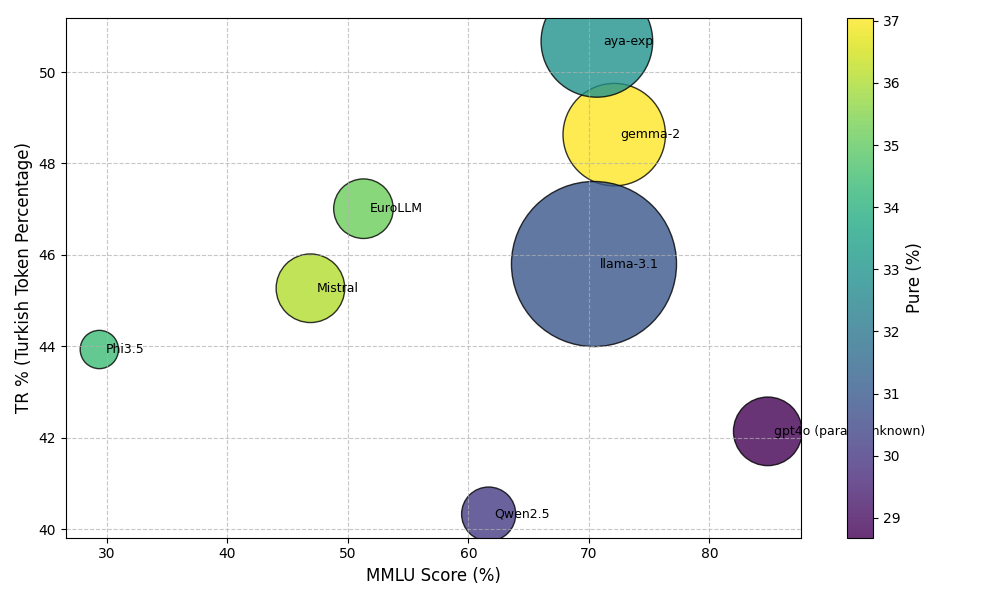
\includegraphics[width=1\textwidth]{model_comparison.png}
    \caption{
    Model Karşılaştırması: MMLU vs TR\%, Parametre Boyutu (gpt4o için bilinmiyor) ve Pure\%
    }
    \label{fig:model_comparison}
\end{figure}

Sonuç olarak, bu bulgular, dilsel uyumun, morfolojik olarak karmaşık ortamlarda aşağı akış görevlerindeki başarıyı büyük ölçüde şekillendirdiğini doğrulamaktadır. Özel olarak uyarlanmış tokenizasyon, daha küçük modellerin etkili bir şekilde rekabet etmesine yardımcı olabilirken, daha büyük veya optimize edilmiş modeller bile tokenizatörleri dilsel olarak uyumlu olmadığında yetersiz kalabilir.

\section{Gelecek Çalışmalar}

Bu çalışma, morfolojik olarak zengin ve düşük kaynaklı diller için optimize edilmiş tokenizatörlerin geliştirilmesine rehberlik eden bir çerçeve sunarak, dilsel bütünlük ve hesaplama verimliliğinin önemini vurgulamaktadır. Araştırma kapsamında geliştirilen çeşitli tokenizatörler, Türkçe gibi morfolojik açıdan karmaşık dillerde promising performans sergilemektedir. Ancak, bu tokenizatörler, bu tür dillerin tokenize edilmesiyle ilgili zorlukların yalnızca başlangıç aşamasını ele almaktadır. Tablo~\ref{tab:future-tokenizers}, \texttt{AhmetSemih/tr\_tokenizer} ve \texttt{aliarda/turkish\_tokenizer} gibi tokenizatörlerin, yüksek Türkçe Token Yüzdeleri (\%TR) ve Saf Token Yüzdeleri (\%Pure) ile dikkat çektiğini göstermektedir.

\begin{table}[H]
\centering
\caption{Tokenizatörlerin İlk Geliştirme Aşamasındaki Performans Metrikleri}
\label{tab:future-tokenizers}
\resizebox{\textwidth}{!}{
\begin{tabular}{|l|c|c|c|c|c|c|c|c|}
\hline
\textbf{Tokenizatör} & \textbf{Sözlük Boyutu} & \textbf{Token Sayısı} & \textbf{Zaman (s)} & \textbf{Benzersiz Tokenlar} & \textbf{Türkçe Tokenlar} & \textbf{\%TR} & \textbf{Saf Tokenlar} & \textbf{\%Pure} \\ \hline
\texttt{alibayram/tr\_tokenizer} & 30,158 & 476,556 & 2.42 & 11,531 & 11,342 & 98.36 & 11,055 & 95.87 \\ \hline
\texttt{AhmetSemih/tr\_tokenizer} & 59,572 & 451,883 & 2.48 & 13,370 & 13,253 & 99.12 & 13,357 & 99.90 \\ \hline
\texttt{aliarda/turkish\_tokenizer\_256k} & 256,000 & 488,267 & 2.51 & 13,631 & 13,351 & 97.95 & 12,981 & 95.23 \\ \hline
\texttt{aliarda/turkish\_tokenizer} & 58,526 & 451,936 & 2.34 & 13,268 & 13,170 & 99.26 & 13,256 & 99.91 \\ \hline
\end{tabular}
}
\end{table}

Bu umut verici sonuçlara rağmen, bu tokenizatörlerin tam potansiyelini ortaya çıkarmak için daha fazla çalışma gerekmektedir. Gelecekteki iyileştirmeler, Türkçe'nin zengin dilbilgisel ve anlamsal yapısını daha iyi yakalamak için gelişmiş morfolojik analiz adımlarının entegrasyonuna odaklanacaktır. Bu adımlar arasında daha sofistike dilbilimsel kuralların entegrasyonu, nadir görülen morfemlerin ele alınması ve bağlama dayalı varyasyonların hesaba katılması yer alabilir. Bu tür geliştirmeler yalnızca dilsel bütünlüğü artırmakla kalmayacak, aynı zamanda tokenizatörlerin çeşitli NLP uygulamaları için kapsamını da genişletecektir.

Ek olarak, tokenizasyon süreçlerini dinamik hale getiren yinelemeli iyileştirme yöntemleri araştırılacaktır. Bu yöntemler arasında, aşağı akış görevleri ve alan spesifik gereksinimlere göre dinamik token üretimi yer alabilir. Örneğin, tokenizatörler, tıbbi, hukuki veya teknik metinler gibi belirli alanlar için ince ayar yapılarak, özel uygulamalarda yüksek performans sağlamaları hedeflenebilir. Ayrıca, denetimsiz ve yarı-denetimli öğrenme yaklaşımlarının geliştirme süreçlerine dahil edilmesi, morfolojik ve anlamsal kapsama alanındaki eksikliklerin giderilmesine yardımcı olacaktır.

Henüz gelişimin erken aşamalarında olmasına rağmen, bu tokenizatörler daha fazla yenilik için sağlam bir temel sunmaktadır. İlk performansları, hedeflenen iyileştirmelerle birlikte, morfolojik olarak zengin dillerin tokenize edilmesinde güçlü ve çok yönlü araçlara dönüşebilecekleri umudunu vermektedir. Bu ek adımların uygulanması ve farklı diller ve görevler üzerinde daha fazla değerlendirme yapılmasıyla, bu araştırma, dilbilimsel açıdan bilgilendirilmiş tokenizasyon için yeni bir standart oluşturmayı ve dil modellerinin kalite ve verimliliğini çeşitli uygulamalarda ileri taşımayı amaçlamaktadır.

\section{Sonuç}

Bu çalışma, tokenizasyon stratejilerini değerlendirmek için kapsamlı bir çerçeve sunarak, dilsel bütünlüğün korunmasının yanı sıra hesaplama verimliliğinin önemini vurgulamaktadır. Token saflığı (\textit{token purity}), Türkçe Token Yüzdesi (TR \%) ve işlem verimliliği gibi metriklere odaklanarak, tokenizasyon stratejilerinin özellikle morfolojik olarak zengin dillerde, Türkçe gibi, model performansı üzerinde önemli bir etkisi olduğunu göstermiştir. Analizlerimiz, parametre boyutunun tek başına performansın kesin bir göstergesi olmadığını ortaya koymuştur. Örneğin, \texttt{gemma-2} (27.2 milyar parametre), Türkçe MMLU değerlendirmelerinde daha büyük bir model olan \texttt{llama-3.1}’i (70.6 milyar parametre) geride bırakarak, tokenizasyonun dil yapısıyla uyumunun kritik rolünü vurgulamıştır. Buna karşılık, genel amaçlı modeller olan \texttt{o200k-gpt4} gibi, kapsamlı optimizasyonlar sayesinde aşağı akış görevlerinde mükemmel sonuçlar elde ederken, daha düşük dilsel bütünlük sergilemiş ve görev odaklı model optimizasyonunun doğal getirdiği ödünleşimlere dikkat çekmiştir. 

Bu bulgular, dilsel korunumu ve hesaplama gereksinimlerini dengeleyen özelleştirilmiş tokenizasyon stratejilerinin, çeşitli dillerde sağlam NLP performansı elde etmek için gerekli olduğunu vurgulamaktadır. Önerilen çerçeve yalnızca Türkçe’ye değil, diğer dillere ve alanlara da uygulanabilir olup, tokenizasyon yöntemlerini optimize etmek ve çok dilli NLP uygulamalarını iyileştirmek için bir temel sunmaktadır. Gelecek araştırmalar, bu çerçeveyi görev özelinde değerlendirmeleri ve diller arası karşılaştırmaları kapsayacak şekilde genişleterek, çeşitli dil bağlamları için tokenizasyon stratejilerini daha da geliştirmeyi hedefleyecektir.

\bibliographystyle{unsrt}
% \bibliographystyle{plain}
\bibliography{tokenizer}

\end{document}